\documentclass[11pt]{article}
\usepackage[small,compact]{titlesec}
\usepackage[margin=0.25in]{geometry}
\usepackage{subcaption}
\usepackage{common}
\title{Practical 2: Classifying Malicious Software}
\author{ Baojia Tong (baojia.tong@cern.ch)\\Yuliya Dovzhenko (dovzhenko@g.harvard.edu)\\Alan Legoallec (alanlegoallec@g.harvard.edu )\\\\Public Repository: https://github.com/tongbaojia/pubcs181}
\begin{document}
\maketitle{}
\paragraph{} In this assignment, we were asked to classify $\sim$ 3000 xml files into 14 malware classes after training on $\sim$ 3000 xml files with known classes. We used this opportunity to explore multiple methods, most notably Random Forest, SVM, MLP, and gradient boosting. We found that Random Forest, combined with feature engineering, produced the best results for this dataset. 
\section{Technical Approach}
We found it helpful to preprocess the data before using it to train the model by extracting additional features and rescaling the data. We also performed cross-validation on the training data in order to tune the details of models before making predictions.
\subsection{Additional Features}
\paragraph{}
We found that the additional features drastically improved our accuracy from 0.666667 to 0.899676. 
The extra features are:       
\begin{itemize}  
\item number of each kind of tag
\item proportion of each kind of tag
\item average number of threads per process
\item average number of systems calls per section
\item average number of system calls per process
 \item total number of tags 
 \end{itemize}
The frequency of different features in the dataset is seen in Figure~\ref{fig:Features}. Notice no extra selection is applied on these features because some malware types are not well represented and we do not want to remove features that are potentially useful for discriminating some specific malwares, even if they often do not appear in other malwares.
\subsection{Handling data}
\paragraph{} We used the train\_test\_split() function from sklearn.model\_selection module to set aside a fraction of our training data as testing data. The testing fraction was between 0.1 and 0.2 for most of our methods. For training the Multilayer Perceptron, we took advantage of the cross-validation included in the fit() function, which is enabled by setting the parameter early\_stopping to True.
\begin{figure}[] 
\centering
    \begin{subfigure}[!t]{0.3\textwidth}
        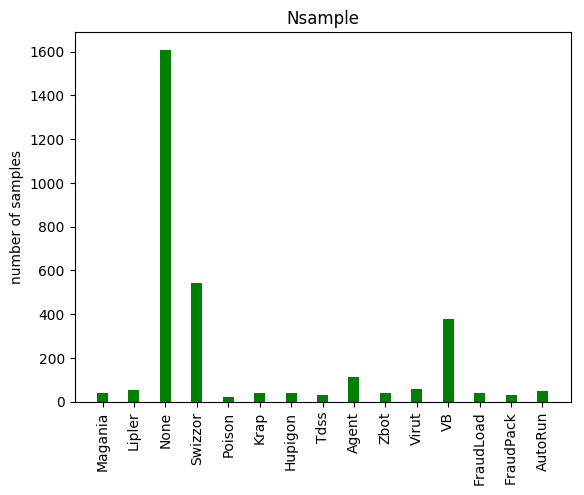
\includegraphics[width=\textwidth]{Plots/Nsample.png}
    \end{subfigure}
        \begin{subfigure}[!t]{0.3\textwidth}
        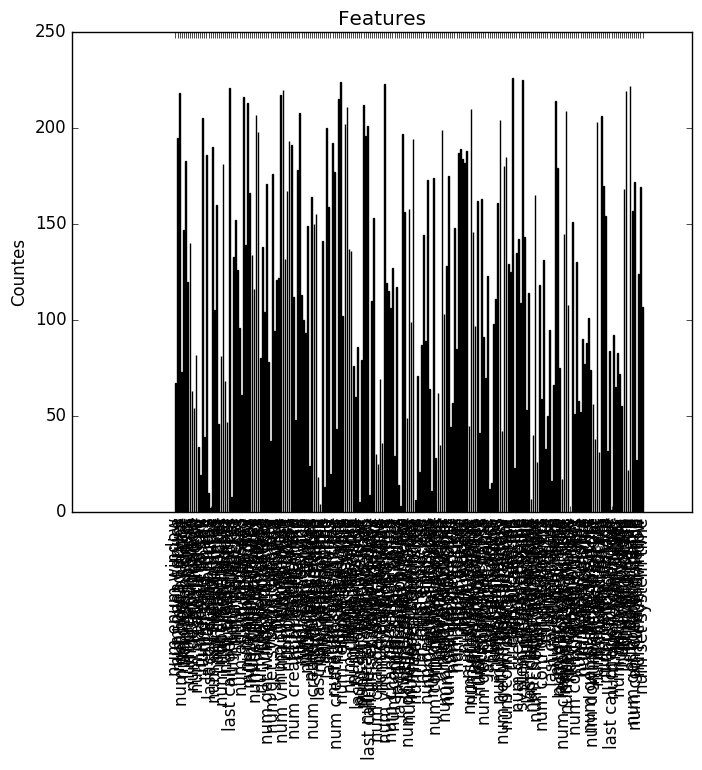
\includegraphics[width=\textwidth]{Plots/Features.png}
    \end{subfigure}
            \begin{subfigure}[!t]{0.3\textwidth}
        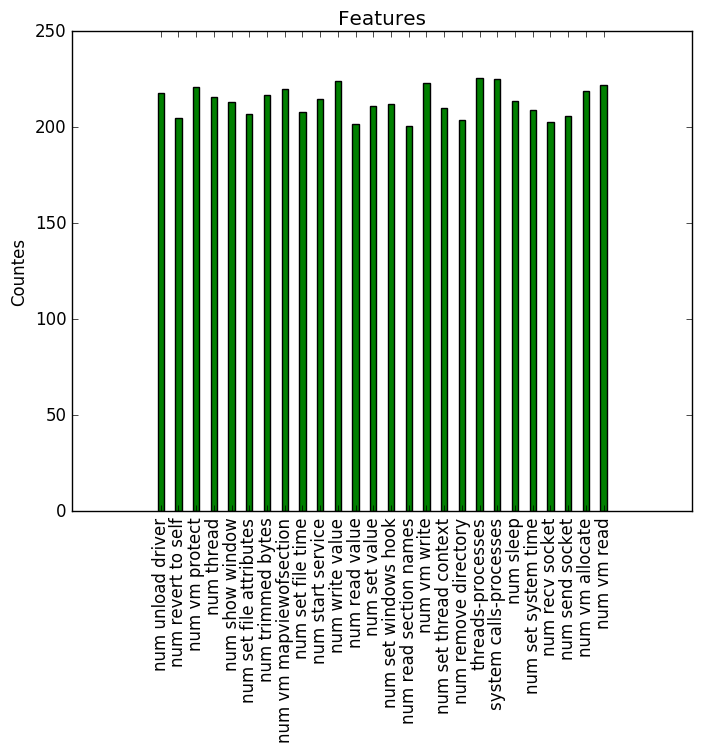
\includegraphics[width=\textwidth]{Plots/Features_top.png}
    \end{subfigure}\\
        \caption{(a) List of malware and their number of samples. Large variation is observed; (b) number of countes for all 227 features (c) top appearing features.}
            \label{fig:Features}
\end{figure}
\paragraph{} Because some columns in our data matrix contain on average larger numbers than other columns, we had to scale the data. This is done automatically in some scikit modules, but it is not done in the MLP fit function. Therefore, we scaled our data using StandardScaler from sklearn.preprocessing library, and we took care to apply the same scaling to the train and test datasets. Ordinarily, we would like all data columns to have 0 mean and 1 standard deviation. However, when working with sparse matrices, adjusting the mean would lead to a drastic increase in the matrix size because many zero entries would be shifted to non-zero values. Therefore, we limited ourselves to enforcing 1 standard deviation. It is possible that converting the data to a dense format and scaling and shifting it may have produced better results. 
\section{Results}
\paragraph{} We explored four different methods and compared the results. Kaggle scores obtained by our methods are summarized in table \ref{tab:results}. The best score is achieved by using a Random Forest. Part of the reason why some models perform better comes from the large number of input features, which could be well captured by the decision tree and random forest, while for SVM and MLP it is more difficult.
  \begin{table}
\centering
\begin{tabular}{llr}
 \toprule
 Model &  & Acc. \\
 \midrule
 \textsc{Baseline} & & 0.70000\\
 \textsc{SVM} & & 0.77526 \\
 \textsc{MLP} & & 0.78211 \\
 \textsc{Decision Tree} & & 0.80632\\
  \textsc{Random Forest} & &0.82421\\
 \bottomrule
\end{tabular}
\caption{\label{tab:results} Summary of our best prediction accuracies on the kaggle test dataset.}
\end{table}
\subsection{Multilayer Perceptron}
\paragraph{}We were interested in comparing the performance of a neural network to other algorithms. We used the Multilayer Perceptron Classifier from the scikit learn module. We found that while MLP beat the baseline, it performed poorly compared to the Random Forest. This may be explained by the small size of the dataset: MLP needs to simultaneously tune many parameters, while each random tree in a forest can have fewer parameters than dimensions in the data and still capture the data well due to the superposition of many random trees.
\paragraph{}To determine the optimal number of parameters in a MLP model, we varied the number of layers and nodes and recorded cross-validation accuracy. Starting with three hidden layers and varying the number of nodes in each layer, we obtained the accuracy values in figure \ref{fig:MLP} (a). Since the accuracy didn't seem to saturate at 20 nodes, we extended our search all the way to 203 nodes, which equals the number of our features. It made very little sense to us to create more nodes than dimensions in the data. Despite small fluctuations, we saw an overall trend where the accuracy increases up to 25 nodes, and then stays approximately constant, shown in figure \ref{fig:MLP} (b). 
\paragraph{}While adding more nodes improved our accuracy, adding layers beyond three actually hurt the performance (see figure \ref{fig:MLP} (c)). This could be a reflection of the true nature of the relationships between different features, or it could simply indicate that the amount of data was insufficient to properly tune increasing numbers of layers. Finally, we experimented with activation functions and optimization methods, and found that the default settings of relu activation and adam optimization were in fact the best ones for this dataset.
\begin{figure}[] 
\centering
    \begin{subfigure}[!t]{0.3\textwidth}
        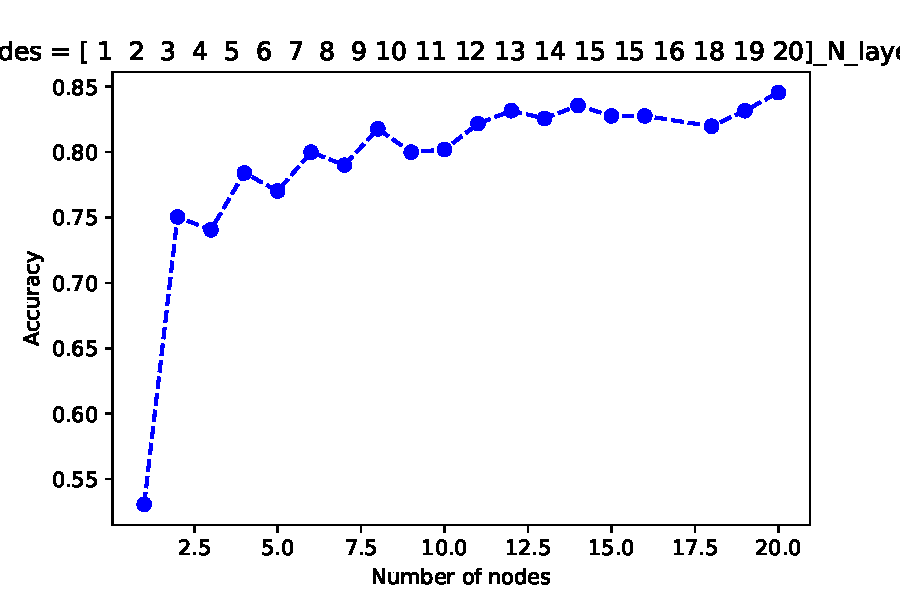
\includegraphics[width=\textwidth]{Plots/Alan_features_N_nodes_1_20_N_layers3.pdf}
    \end{subfigure}
        \begin{subfigure}[!t]{0.3\textwidth}
        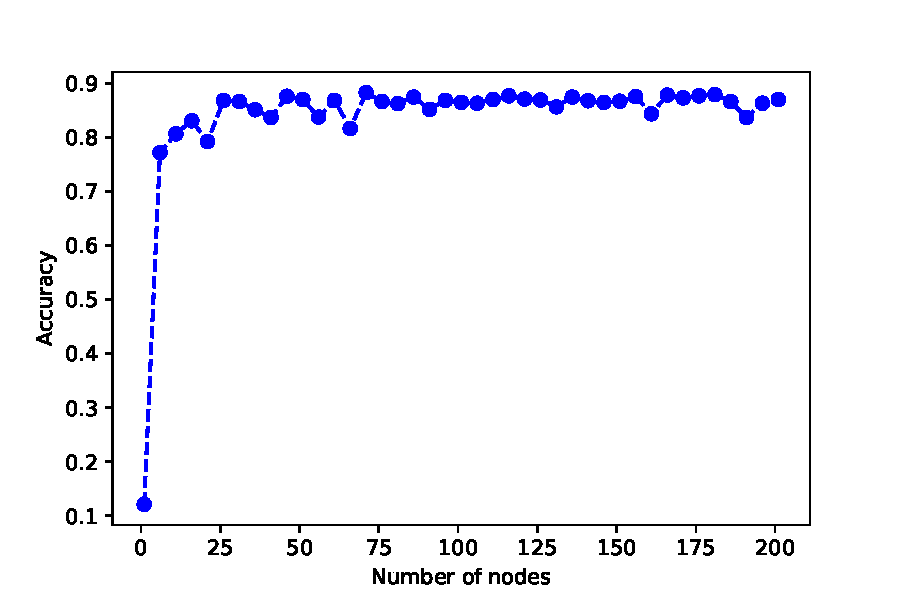
\includegraphics[width=\textwidth]{Plots/Alan_features_N_nodes_6-201_N_layers3.pdf}
    \end{subfigure}
            \begin{subfigure}[!t]{0.3\textwidth}
        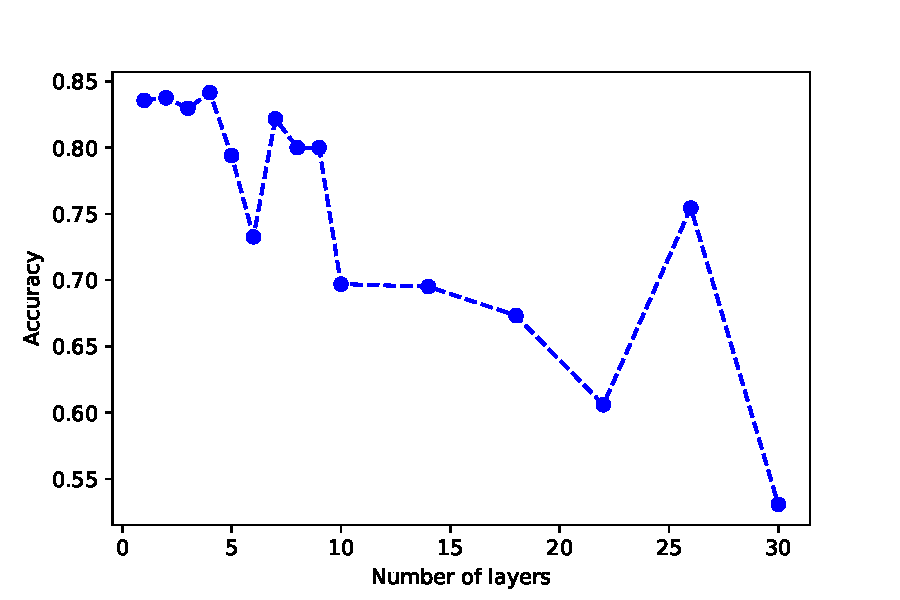
\includegraphics[width=\textwidth]{Plots/Alan_features_N_nodes_50_N_layers_1_30.pdf}
    \end{subfigure}\\
        \caption{Accuracy achieved with a Multilayer Perceptron algorithm (a) with three hidden layers and up to 20 nodes in each layer; (b) with three hidden layers and up to 203 nodes in each layer (equal to the number of features in the data) (c) with 50 nodes, and a variable number of hidden layers between 1 and 30.}
            \label{fig:MLP}
\end{figure}
\paragraph{}With a small dataset, it is important to avoid overfitting. With this in mind, we explored regularization within the MLP algorithm. This is done by changing the value of a constant $\alpha$, with larger $\alpha$ meaning larger penalty for overfitting. Interestingly, changing $\alpha$ by multiple orders of magnitude had no effect on our model's accuracy. These data are summarized in table \ref{tab:alpha}.
\begin{table}
\centering
\begin{tabular}{llr}
 \toprule
$\alpha$ &  & Accuracy \\
 \midrule
 \textsc{1e-5} & & 0.880259\\
 \textsc{1e-4} & & 0.899676 \\
 \textsc{1e-3} & & 0.880259 \\
 \textsc{1e-2} & & 0.883495\\
 \bottomrule
\end{tabular}
\caption{\label{tab:alpha} The effect of regularization (quantified by a penalty constant $\alpha$) on the accuracy of MLP predictions.}
\end{table}
\subsection{Decision Tree}
\paragraph{}Decision Tree method is also tested. To investigate the performance, different maximum depth, maximum number of features, and maximum number of leaf nodes are tested in order, as can be seen in Figure~\ref{fig:DT}. A decision tree with depth greater than 7, with feature greater than 3, and with leaf nodes greater than 50 seems to give us good performance. Interestingly, adding more depth, features or nodes doesn't seem to help us improve the performance. This could be because our training information is limited. If a large number of maximum depth, features or nodes are used, the risk of overtraining will be significant.
\begin{figure}[] 
\centering
    \begin{subfigure}[!t]{0.3\textwidth}
        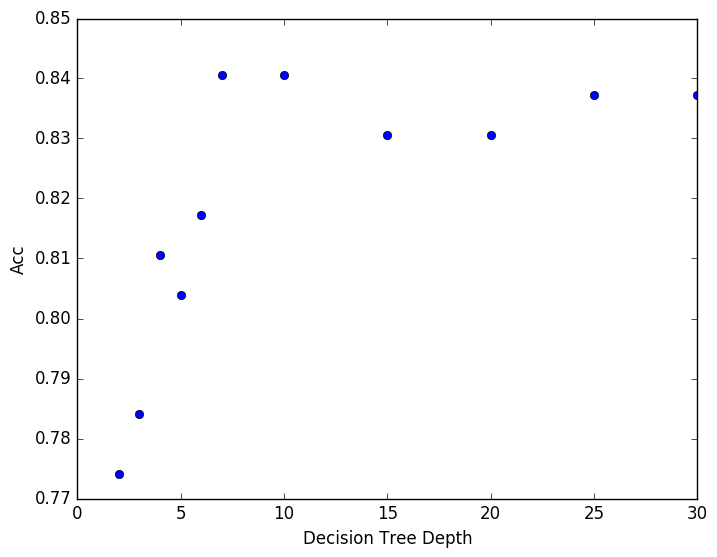
\includegraphics[width=\textwidth]{Plots/DT_depth.png}
    \end{subfigure}
        \begin{subfigure}[!t]{0.3\textwidth}
        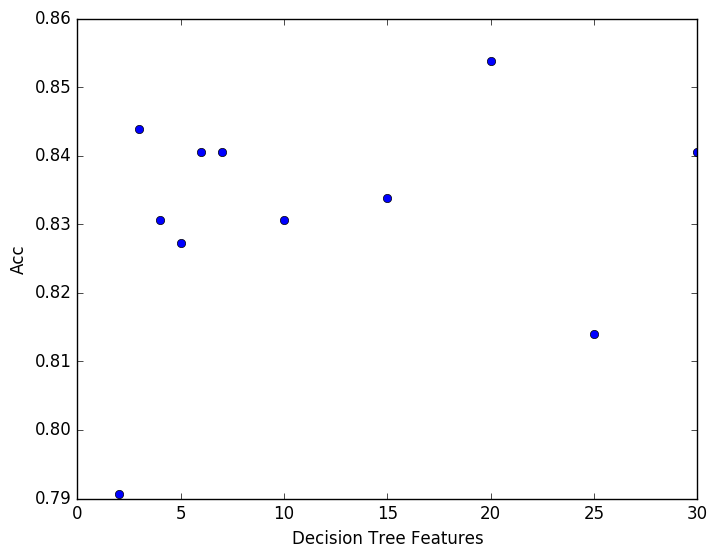
\includegraphics[width=\textwidth]{Plots/DT_feature.png}
    \end{subfigure}
            \begin{subfigure}[!t]{0.3\textwidth}
        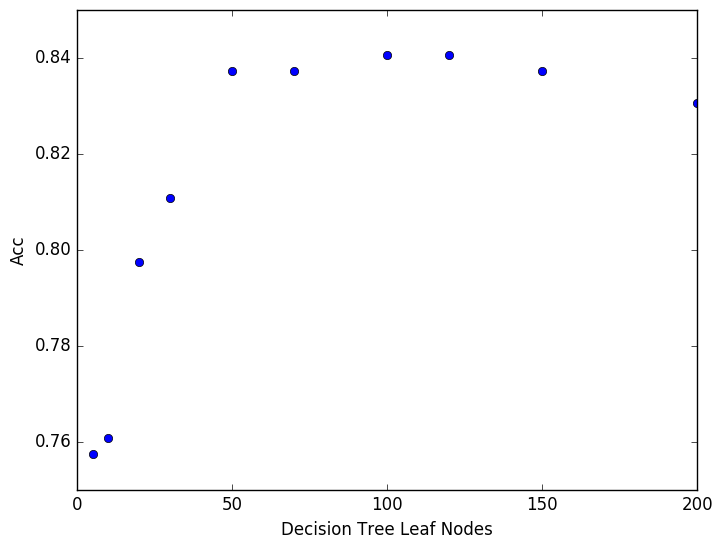
\includegraphics[width=\textwidth]{Plots/DT_leafnodes.png}
    \end{subfigure}\\
        \caption{Accuracy achieved with a Decision Tree algorithm (a) with different number of depth; (b) with depth 10 and different number of max features (c)  with depth 10, maximum features 5, and different number of of leaf nodes.}
            \label{fig:DT}
\end{figure}

\section{Discussion} 
\paragraph{}We found that the best results are achieved through a combination of feature engineering and relatively simple methods like the Random Forest. We suspect that simpler methods (with fewer parameters) perform so well here because the data set is small. A neural network would require much more data to tune the parameters.
\paragraph{}Different malware classes appear with different frequencies in the training data set. If given more time, we would explore how this affects our accuracy by preselecting particular numbers of data points from each class. Also, more features can possibly be extracted from the information contained in the subprocess commands, which could help further improve the performance. 
\paragraph{}Since the data are sparse, we could also apply Principal Component Analysis and then examine the feature composition of each component. This would help us gain intuition about the different malware classes. It may also be interesting to firstly train a classifier to distinguish the malware and the None type, and then a second classifier to further classify the different malware types. 
\paragraph{}Given our testing score is significantly higher than the kaggle final score, overfitting seems to exist. Bagging will help in this case to reduce the variance.


\end{document}

